% Created by tikzDevice version 0.12.6 on 2026-07-31 23:28:08
% !TEX encoding = UTF-8 Unicode
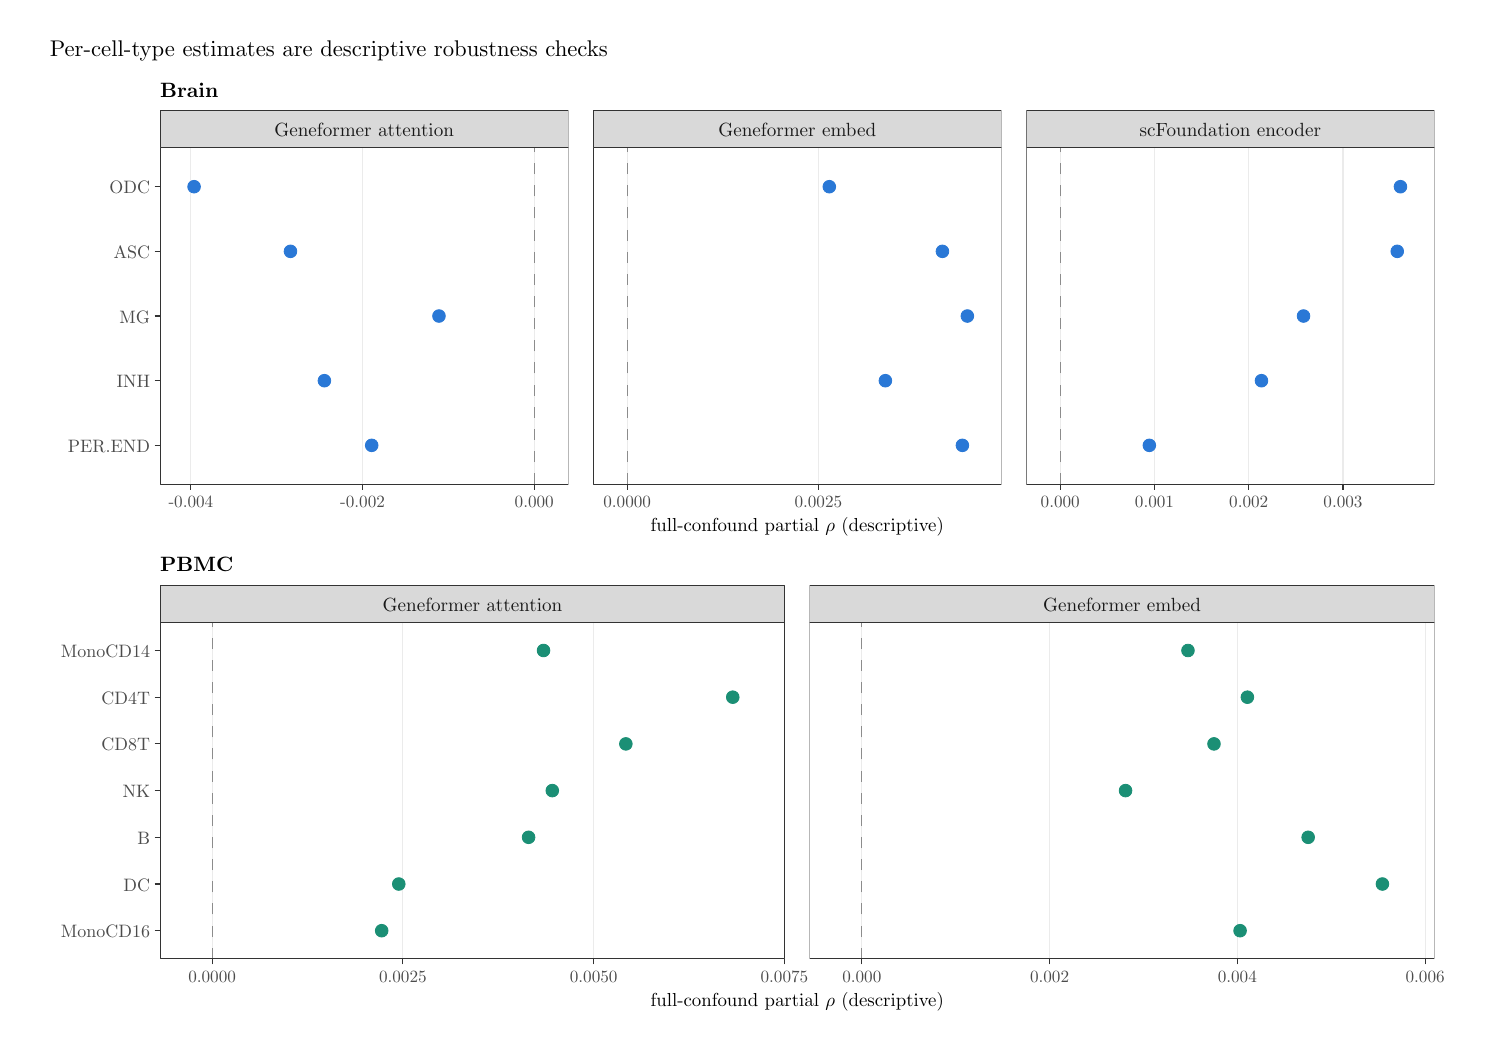
\begin{tikzpicture}[x=1pt,y=1pt]
\definecolor{fillColor}{RGB}{255,255,255}
\path[use as bounding box,fill=fillColor,fill opacity=0.00] (0,0) rectangle (520.34,361.35);
\begin{scope}
\path[clip] (  0.00,  0.00) rectangle (520.34,361.35);
\definecolor{drawColor}{RGB}{255,255,255}
\definecolor{fillColor}{RGB}{255,255,255}

\path[draw=drawColor,line width= 0.4pt,line join=round,line cap=round,fill=fillColor] ( -0.00,  0.00) rectangle (520.34,361.35);
\end{scope}
\begin{scope}
\path[clip] (  4.00,174.49) rectangle (514.34,345.97);
\definecolor{drawColor}{RGB}{255,255,255}
\definecolor{fillColor}{RGB}{255,255,255}

\path[draw=drawColor,line width= 0.4pt,line join=round,line cap=round,fill=fillColor] (  4.00,174.49) rectangle (514.34,345.97);
\end{scope}
\begin{scope}
\path[clip] (  4.00,  3.00) rectangle (514.34,174.49);
\definecolor{drawColor}{RGB}{255,255,255}
\definecolor{fillColor}{RGB}{255,255,255}

\path[draw=drawColor,line width= 0.4pt,line join=round,line cap=round,fill=fillColor] (  4.00,  3.00) rectangle (514.34,174.49);
\end{scope}
\begin{scope}
\path[clip] ( 47.84,196.40) rectangle (195.34,317.90);
\definecolor{fillColor}{RGB}{255,255,255}

\path[fill=fillColor] ( 47.84,196.40) rectangle (195.34,317.90);
\definecolor{drawColor}{gray}{0.92}

\path[draw=drawColor,line width= 0.4pt,line join=round] ( 58.99,196.40) --
	( 58.99,317.90);

\path[draw=drawColor,line width= 0.4pt,line join=round] (121.02,196.40) --
	(121.02,317.90);

\path[draw=drawColor,line width= 0.4pt,line join=round] (183.05,196.40) --
	(183.05,317.90);
\definecolor{drawColor}{gray}{0.55}

\path[draw=drawColor,line width= 0.4pt,dash pattern=on 4pt off 4pt ,line join=round] (183.05,196.40) -- (183.05,317.90);
\definecolor{drawColor}{RGB}{42,120,214}
\definecolor{fillColor}{RGB}{42,120,214}

\path[draw=drawColor,line width= 0.3pt,line join=round,line cap=round,fill=fillColor] ( 60.13,303.88) circle (  2.29);

\path[draw=drawColor,line width= 0.3pt,line join=round,line cap=round,fill=fillColor] ( 94.96,280.52) circle (  2.29);

\path[draw=drawColor,line width= 0.3pt,line join=round,line cap=round,fill=fillColor] (148.62,257.15) circle (  2.29);

\path[draw=drawColor,line width= 0.3pt,line join=round,line cap=round,fill=fillColor] (107.22,233.78) circle (  2.29);

\path[draw=drawColor,line width= 0.3pt,line join=round,line cap=round,fill=fillColor] (124.31,210.42) circle (  2.29);
\definecolor{drawColor}{gray}{0.20}

\path[draw=drawColor,line width= 0.4pt,line join=round,line cap=round] ( 47.84,196.40) rectangle (195.34,317.90);
\end{scope}
\begin{scope}
\path[clip] (204.34,196.40) rectangle (351.84,317.90);
\definecolor{fillColor}{RGB}{255,255,255}

\path[fill=fillColor] (204.34,196.40) rectangle (351.84,317.90);
\definecolor{drawColor}{gray}{0.92}

\path[draw=drawColor,line width= 0.4pt,line join=round] (216.63,196.40) --
	(216.63,317.90);

\path[draw=drawColor,line width= 0.4pt,line join=round] (285.72,196.40) --
	(285.72,317.90);
\definecolor{drawColor}{gray}{0.55}

\path[draw=drawColor,line width= 0.4pt,dash pattern=on 4pt off 4pt ,line join=round] (216.63,196.40) -- (216.63,317.90);
\definecolor{drawColor}{RGB}{42,120,214}
\definecolor{fillColor}{RGB}{42,120,214}

\path[draw=drawColor,line width= 0.3pt,line join=round,line cap=round,fill=fillColor] (289.67,303.88) circle (  2.29);

\path[draw=drawColor,line width= 0.3pt,line join=round,line cap=round,fill=fillColor] (330.54,280.52) circle (  2.29);

\path[draw=drawColor,line width= 0.3pt,line join=round,line cap=round,fill=fillColor] (339.55,257.15) circle (  2.29);

\path[draw=drawColor,line width= 0.3pt,line join=round,line cap=round,fill=fillColor] (309.93,233.78) circle (  2.29);

\path[draw=drawColor,line width= 0.3pt,line join=round,line cap=round,fill=fillColor] (337.76,210.42) circle (  2.29);
\definecolor{drawColor}{gray}{0.20}

\path[draw=drawColor,line width= 0.4pt,line join=round,line cap=round] (204.34,196.40) rectangle (351.84,317.90);
\end{scope}
\begin{scope}
\path[clip] (360.84,196.40) rectangle (508.34,317.90);
\definecolor{fillColor}{RGB}{255,255,255}

\path[fill=fillColor] (360.84,196.40) rectangle (508.34,317.90);
\definecolor{drawColor}{gray}{0.92}

\path[draw=drawColor,line width= 0.4pt,line join=round] (373.13,196.40) --
	(373.13,317.90);

\path[draw=drawColor,line width= 0.4pt,line join=round] (407.18,196.40) --
	(407.18,317.90);

\path[draw=drawColor,line width= 0.4pt,line join=round] (441.23,196.40) --
	(441.23,317.90);

\path[draw=drawColor,line width= 0.4pt,line join=round] (475.28,196.40) --
	(475.28,317.90);
\definecolor{drawColor}{gray}{0.55}

\path[draw=drawColor,line width= 0.4pt,dash pattern=on 4pt off 4pt ,line join=round] (373.13,196.40) -- (373.13,317.90);
\definecolor{drawColor}{RGB}{42,120,214}
\definecolor{fillColor}{RGB}{42,120,214}

\path[draw=drawColor,line width= 0.3pt,line join=round,line cap=round,fill=fillColor] (496.05,303.88) circle (  2.29);

\path[draw=drawColor,line width= 0.3pt,line join=round,line cap=round,fill=fillColor] (494.89,280.52) circle (  2.29);

\path[draw=drawColor,line width= 0.3pt,line join=round,line cap=round,fill=fillColor] (461.02,257.15) circle (  2.29);

\path[draw=drawColor,line width= 0.3pt,line join=round,line cap=round,fill=fillColor] (445.83,233.78) circle (  2.29);

\path[draw=drawColor,line width= 0.3pt,line join=round,line cap=round,fill=fillColor] (405.31,210.42) circle (  2.29);
\definecolor{drawColor}{gray}{0.20}

\path[draw=drawColor,line width= 0.4pt,line join=round,line cap=round] (360.84,196.40) rectangle (508.34,317.90);
\end{scope}
\begin{scope}
\path[clip] ( 47.84,317.90) rectangle (195.34,331.38);
\definecolor{drawColor}{gray}{0.20}
\definecolor{fillColor}{gray}{0.85}

\path[draw=drawColor,line width= 0.4pt,line join=round,line cap=round,fill=fillColor] ( 47.84,317.90) rectangle (195.34,331.38);
\definecolor{drawColor}{gray}{0.10}

\node[text=drawColor,anchor=base,inner sep=0pt, outer sep=0pt, scale=  0.69] at (121.59,321.95) {Geneformer attention};
\end{scope}
\begin{scope}
\path[clip] (204.34,317.90) rectangle (351.84,331.38);
\definecolor{drawColor}{gray}{0.20}
\definecolor{fillColor}{gray}{0.85}

\path[draw=drawColor,line width= 0.4pt,line join=round,line cap=round,fill=fillColor] (204.34,317.90) rectangle (351.84,331.38);
\definecolor{drawColor}{gray}{0.10}

\node[text=drawColor,anchor=base,inner sep=0pt, outer sep=0pt, scale=  0.69] at (278.09,321.95) {Geneformer embed};
\end{scope}
\begin{scope}
\path[clip] (360.84,317.90) rectangle (508.34,331.38);
\definecolor{drawColor}{gray}{0.20}
\definecolor{fillColor}{gray}{0.85}

\path[draw=drawColor,line width= 0.4pt,line join=round,line cap=round,fill=fillColor] (360.84,317.90) rectangle (508.34,331.38);
\definecolor{drawColor}{gray}{0.10}

\node[text=drawColor,anchor=base,inner sep=0pt, outer sep=0pt, scale=  0.69] at (434.59,321.95) {scFoundation encoder};
\end{scope}
\begin{scope}
\path[clip] (  0.00,  0.00) rectangle (520.34,361.35);
\definecolor{drawColor}{gray}{0.20}

\path[draw=drawColor,line width= 0.4pt,line join=round] ( 58.99,194.40) --
	( 58.99,196.40);

\path[draw=drawColor,line width= 0.4pt,line join=round] (121.02,194.40) --
	(121.02,196.40);

\path[draw=drawColor,line width= 0.4pt,line join=round] (183.05,194.40) --
	(183.05,196.40);
\end{scope}
\begin{scope}
\path[clip] (  0.00,  0.00) rectangle (520.34,361.35);
\definecolor{drawColor}{gray}{0.30}

\node[text=drawColor,anchor=base,inner sep=0pt, outer sep=0pt, scale=  0.62] at ( 58.99,187.97) {-0.004};

\node[text=drawColor,anchor=base,inner sep=0pt, outer sep=0pt, scale=  0.62] at (121.02,187.97) {-0.002};

\node[text=drawColor,anchor=base,inner sep=0pt, outer sep=0pt, scale=  0.62] at (183.05,187.97) {0.000};
\end{scope}
\begin{scope}
\path[clip] (  0.00,  0.00) rectangle (520.34,361.35);
\definecolor{drawColor}{gray}{0.20}

\path[draw=drawColor,line width= 0.4pt,line join=round] (216.63,194.40) --
	(216.63,196.40);

\path[draw=drawColor,line width= 0.4pt,line join=round] (285.72,194.40) --
	(285.72,196.40);
\end{scope}
\begin{scope}
\path[clip] (  0.00,  0.00) rectangle (520.34,361.35);
\definecolor{drawColor}{gray}{0.30}

\node[text=drawColor,anchor=base,inner sep=0pt, outer sep=0pt, scale=  0.62] at (216.63,187.97) {0.0000};

\node[text=drawColor,anchor=base,inner sep=0pt, outer sep=0pt, scale=  0.62] at (285.72,187.97) {0.0025};
\end{scope}
\begin{scope}
\path[clip] (  0.00,  0.00) rectangle (520.34,361.35);
\definecolor{drawColor}{gray}{0.20}

\path[draw=drawColor,line width= 0.4pt,line join=round] (373.13,194.40) --
	(373.13,196.40);

\path[draw=drawColor,line width= 0.4pt,line join=round] (407.18,194.40) --
	(407.18,196.40);

\path[draw=drawColor,line width= 0.4pt,line join=round] (441.23,194.40) --
	(441.23,196.40);

\path[draw=drawColor,line width= 0.4pt,line join=round] (475.28,194.40) --
	(475.28,196.40);
\end{scope}
\begin{scope}
\path[clip] (  0.00,  0.00) rectangle (520.34,361.35);
\definecolor{drawColor}{gray}{0.30}

\node[text=drawColor,anchor=base,inner sep=0pt, outer sep=0pt, scale=  0.62] at (373.13,187.97) {0.000};

\node[text=drawColor,anchor=base,inner sep=0pt, outer sep=0pt, scale=  0.62] at (407.18,187.97) {0.001};

\node[text=drawColor,anchor=base,inner sep=0pt, outer sep=0pt, scale=  0.62] at (441.23,187.97) {0.002};

\node[text=drawColor,anchor=base,inner sep=0pt, outer sep=0pt, scale=  0.62] at (475.28,187.97) {0.003};
\end{scope}
\begin{scope}
\path[clip] (  0.00,  0.00) rectangle (520.34,361.35);
\definecolor{drawColor}{gray}{0.30}

\node[text=drawColor,anchor=base east,inner sep=0pt, outer sep=0pt, scale=  0.65] at ( 44.24,207.86) {PER.END};

\node[text=drawColor,anchor=base east,inner sep=0pt, outer sep=0pt, scale=  0.65] at ( 44.24,231.23) {INH};

\node[text=drawColor,anchor=base east,inner sep=0pt, outer sep=0pt, scale=  0.65] at ( 44.24,254.60) {MG};

\node[text=drawColor,anchor=base east,inner sep=0pt, outer sep=0pt, scale=  0.65] at ( 44.24,277.96) {ASC};

\node[text=drawColor,anchor=base east,inner sep=0pt, outer sep=0pt, scale=  0.65] at ( 44.24,301.33) {ODC};
\end{scope}
\begin{scope}
\path[clip] (  0.00,  0.00) rectangle (520.34,361.35);
\definecolor{drawColor}{gray}{0.20}

\path[draw=drawColor,line width= 0.4pt,line join=round] ( 45.84,210.42) --
	( 47.84,210.42);

\path[draw=drawColor,line width= 0.4pt,line join=round] ( 45.84,233.78) --
	( 47.84,233.78);

\path[draw=drawColor,line width= 0.4pt,line join=round] ( 45.84,257.15) --
	( 47.84,257.15);

\path[draw=drawColor,line width= 0.4pt,line join=round] ( 45.84,280.52) --
	( 47.84,280.52);

\path[draw=drawColor,line width= 0.4pt,line join=round] ( 45.84,303.88) --
	( 47.84,303.88);
\end{scope}
\begin{scope}
\path[clip] (  0.00,  0.00) rectangle (520.34,361.35);
\definecolor{drawColor}{RGB}{0,0,0}

\node[text=drawColor,anchor=base,inner sep=0pt, outer sep=0pt, scale=  0.68] at (278.09,179.15) {full-confound partial $\rho$ (descriptive)};
\end{scope}
\begin{scope}
\path[clip] (  0.00,  0.00) rectangle (520.34,361.35);
\definecolor{drawColor}{RGB}{0,0,0}

\node[text=drawColor,anchor=base west,inner sep=0pt, outer sep=0pt, scale=  0.75] at ( 47.84,336.19) {\bfseries Brain};
\end{scope}
\begin{scope}
\path[clip] ( 47.84, 24.91) rectangle (273.59,146.42);
\definecolor{fillColor}{RGB}{255,255,255}

\path[fill=fillColor] ( 47.84, 24.91) rectangle (273.59,146.42);
\definecolor{drawColor}{gray}{0.92}

\path[draw=drawColor,line width= 0.4pt,line join=round] ( 66.65, 24.91) --
	( 66.65,146.42);

\path[draw=drawColor,line width= 0.4pt,line join=round] (135.59, 24.91) --
	(135.59,146.42);

\path[draw=drawColor,line width= 0.4pt,line join=round] (204.52, 24.91) --
	(204.52,146.42);

\path[draw=drawColor,line width= 0.4pt,line join=round] (273.45, 24.91) --
	(273.45,146.42);
\definecolor{drawColor}{gray}{0.55}

\path[draw=drawColor,line width= 0.4pt,dash pattern=on 4pt off 4pt ,line join=round] ( 66.65, 24.91) -- ( 66.65,146.42);
\definecolor{drawColor}{RGB}{27,143,117}
\definecolor{fillColor}{RGB}{27,143,117}

\path[draw=drawColor,line width= 0.3pt,line join=round,line cap=round,fill=fillColor] (186.40,136.29) circle (  2.29);

\path[draw=drawColor,line width= 0.3pt,line join=round,line cap=round,fill=fillColor] (254.78,119.42) circle (  2.29);

\path[draw=drawColor,line width= 0.3pt,line join=round,line cap=round,fill=fillColor] (216.15,102.54) circle (  2.29);

\path[draw=drawColor,line width= 0.3pt,line join=round,line cap=round,fill=fillColor] (189.57, 85.66) circle (  2.29);

\path[draw=drawColor,line width= 0.3pt,line join=round,line cap=round,fill=fillColor] (181.00, 68.79) circle (  2.29);

\path[draw=drawColor,line width= 0.3pt,line join=round,line cap=round,fill=fillColor] (134.10, 51.91) circle (  2.29);

\path[draw=drawColor,line width= 0.3pt,line join=round,line cap=round,fill=fillColor] (127.92, 35.04) circle (  2.29);
\definecolor{drawColor}{gray}{0.20}

\path[draw=drawColor,line width= 0.4pt,line join=round,line cap=round] ( 47.84, 24.91) rectangle (273.59,146.42);
\end{scope}
\begin{scope}
\path[clip] (282.59, 24.91) rectangle (508.34,146.42);
\definecolor{fillColor}{RGB}{255,255,255}

\path[fill=fillColor] (282.59, 24.91) rectangle (508.34,146.42);
\definecolor{drawColor}{gray}{0.92}

\path[draw=drawColor,line width= 0.4pt,line join=round] (301.41, 24.91) --
	(301.41,146.42);

\path[draw=drawColor,line width= 0.4pt,line join=round] (369.26, 24.91) --
	(369.26,146.42);

\path[draw=drawColor,line width= 0.4pt,line join=round] (437.11, 24.91) --
	(437.11,146.42);

\path[draw=drawColor,line width= 0.4pt,line join=round] (504.97, 24.91) --
	(504.97,146.42);
\definecolor{drawColor}{gray}{0.55}

\path[draw=drawColor,line width= 0.4pt,dash pattern=on 4pt off 4pt ,line join=round] (301.41, 24.91) -- (301.41,146.42);
\definecolor{drawColor}{RGB}{27,143,117}
\definecolor{fillColor}{RGB}{27,143,117}

\path[draw=drawColor,line width= 0.3pt,line join=round,line cap=round,fill=fillColor] (419.27,136.29) circle (  2.29);

\path[draw=drawColor,line width= 0.3pt,line join=round,line cap=round,fill=fillColor] (440.74,119.42) circle (  2.29);

\path[draw=drawColor,line width= 0.3pt,line join=round,line cap=round,fill=fillColor] (428.67,102.54) circle (  2.29);

\path[draw=drawColor,line width= 0.3pt,line join=round,line cap=round,fill=fillColor] (396.71, 85.66) circle (  2.29);

\path[draw=drawColor,line width= 0.3pt,line join=round,line cap=round,fill=fillColor] (462.70, 68.79) circle (  2.29);

\path[draw=drawColor,line width= 0.3pt,line join=round,line cap=round,fill=fillColor] (489.53, 51.91) circle (  2.29);

\path[draw=drawColor,line width= 0.3pt,line join=round,line cap=round,fill=fillColor] (438.10, 35.04) circle (  2.29);
\definecolor{drawColor}{gray}{0.20}

\path[draw=drawColor,line width= 0.4pt,line join=round,line cap=round] (282.59, 24.91) rectangle (508.34,146.42);
\end{scope}
\begin{scope}
\path[clip] ( 47.84,146.42) rectangle (273.59,159.89);
\definecolor{drawColor}{gray}{0.20}
\definecolor{fillColor}{gray}{0.85}

\path[draw=drawColor,line width= 0.4pt,line join=round,line cap=round,fill=fillColor] ( 47.84,146.42) rectangle (273.59,159.89);
\definecolor{drawColor}{gray}{0.10}

\node[text=drawColor,anchor=base,inner sep=0pt, outer sep=0pt, scale=  0.69] at (160.72,150.46) {Geneformer attention};
\end{scope}
\begin{scope}
\path[clip] (282.59,146.42) rectangle (508.34,159.89);
\definecolor{drawColor}{gray}{0.20}
\definecolor{fillColor}{gray}{0.85}

\path[draw=drawColor,line width= 0.4pt,line join=round,line cap=round,fill=fillColor] (282.59,146.42) rectangle (508.34,159.89);
\definecolor{drawColor}{gray}{0.10}

\node[text=drawColor,anchor=base,inner sep=0pt, outer sep=0pt, scale=  0.69] at (395.47,150.46) {Geneformer embed};
\end{scope}
\begin{scope}
\path[clip] (  0.00,  0.00) rectangle (520.34,361.35);
\definecolor{drawColor}{gray}{0.20}

\path[draw=drawColor,line width= 0.4pt,line join=round] ( 66.65, 22.91) --
	( 66.65, 24.91);

\path[draw=drawColor,line width= 0.4pt,line join=round] (135.59, 22.91) --
	(135.59, 24.91);

\path[draw=drawColor,line width= 0.4pt,line join=round] (204.52, 22.91) --
	(204.52, 24.91);

\path[draw=drawColor,line width= 0.4pt,line join=round] (273.45, 22.91) --
	(273.45, 24.91);
\end{scope}
\begin{scope}
\path[clip] (  0.00,  0.00) rectangle (520.34,361.35);
\definecolor{drawColor}{gray}{0.30}

\node[text=drawColor,anchor=base,inner sep=0pt, outer sep=0pt, scale=  0.62] at ( 66.65, 16.49) {0.0000};

\node[text=drawColor,anchor=base,inner sep=0pt, outer sep=0pt, scale=  0.62] at (135.59, 16.49) {0.0025};

\node[text=drawColor,anchor=base,inner sep=0pt, outer sep=0pt, scale=  0.62] at (204.52, 16.49) {0.0050};

\node[text=drawColor,anchor=base,inner sep=0pt, outer sep=0pt, scale=  0.62] at (273.45, 16.49) {0.0075};
\end{scope}
\begin{scope}
\path[clip] (  0.00,  0.00) rectangle (520.34,361.35);
\definecolor{drawColor}{gray}{0.20}

\path[draw=drawColor,line width= 0.4pt,line join=round] (301.41, 22.91) --
	(301.41, 24.91);

\path[draw=drawColor,line width= 0.4pt,line join=round] (369.26, 22.91) --
	(369.26, 24.91);

\path[draw=drawColor,line width= 0.4pt,line join=round] (437.11, 22.91) --
	(437.11, 24.91);

\path[draw=drawColor,line width= 0.4pt,line join=round] (504.97, 22.91) --
	(504.97, 24.91);
\end{scope}
\begin{scope}
\path[clip] (  0.00,  0.00) rectangle (520.34,361.35);
\definecolor{drawColor}{gray}{0.30}

\node[text=drawColor,anchor=base,inner sep=0pt, outer sep=0pt, scale=  0.62] at (301.41, 16.49) {0.000};

\node[text=drawColor,anchor=base,inner sep=0pt, outer sep=0pt, scale=  0.62] at (369.26, 16.49) {0.002};

\node[text=drawColor,anchor=base,inner sep=0pt, outer sep=0pt, scale=  0.62] at (437.11, 16.49) {0.004};

\node[text=drawColor,anchor=base,inner sep=0pt, outer sep=0pt, scale=  0.62] at (504.97, 16.49) {0.006};
\end{scope}
\begin{scope}
\path[clip] (  0.00,  0.00) rectangle (520.34,361.35);
\definecolor{drawColor}{gray}{0.30}

\node[text=drawColor,anchor=base east,inner sep=0pt, outer sep=0pt, scale=  0.65] at ( 44.24, 32.48) {MonoCD16};

\node[text=drawColor,anchor=base east,inner sep=0pt, outer sep=0pt, scale=  0.65] at ( 44.24, 49.36) {DC};

\node[text=drawColor,anchor=base east,inner sep=0pt, outer sep=0pt, scale=  0.65] at ( 44.24, 66.23) {B};

\node[text=drawColor,anchor=base east,inner sep=0pt, outer sep=0pt, scale=  0.65] at ( 44.24, 83.11) {NK};

\node[text=drawColor,anchor=base east,inner sep=0pt, outer sep=0pt, scale=  0.65] at ( 44.24, 99.99) {CD8T};

\node[text=drawColor,anchor=base east,inner sep=0pt, outer sep=0pt, scale=  0.65] at ( 44.24,116.86) {CD4T};

\node[text=drawColor,anchor=base east,inner sep=0pt, outer sep=0pt, scale=  0.65] at ( 44.24,133.74) {MonoCD14};
\end{scope}
\begin{scope}
\path[clip] (  0.00,  0.00) rectangle (520.34,361.35);
\definecolor{drawColor}{gray}{0.20}

\path[draw=drawColor,line width= 0.4pt,line join=round] ( 45.84, 35.04) --
	( 47.84, 35.04);

\path[draw=drawColor,line width= 0.4pt,line join=round] ( 45.84, 51.91) --
	( 47.84, 51.91);

\path[draw=drawColor,line width= 0.4pt,line join=round] ( 45.84, 68.79) --
	( 47.84, 68.79);

\path[draw=drawColor,line width= 0.4pt,line join=round] ( 45.84, 85.66) --
	( 47.84, 85.66);

\path[draw=drawColor,line width= 0.4pt,line join=round] ( 45.84,102.54) --
	( 47.84,102.54);

\path[draw=drawColor,line width= 0.4pt,line join=round] ( 45.84,119.42) --
	( 47.84,119.42);

\path[draw=drawColor,line width= 0.4pt,line join=round] ( 45.84,136.29) --
	( 47.84,136.29);
\end{scope}
\begin{scope}
\path[clip] (  0.00,  0.00) rectangle (520.34,361.35);
\definecolor{drawColor}{RGB}{0,0,0}

\node[text=drawColor,anchor=base,inner sep=0pt, outer sep=0pt, scale=  0.68] at (278.09,  7.66) {full-confound partial $\rho$ (descriptive)};
\end{scope}
\begin{scope}
\path[clip] (  0.00,  0.00) rectangle (520.34,361.35);
\definecolor{drawColor}{RGB}{0,0,0}

\node[text=drawColor,anchor=base west,inner sep=0pt, outer sep=0pt, scale=  0.75] at ( 47.84,164.71) {\bfseries PBMC};
\end{scope}
\begin{scope}
\path[clip] (  0.00,  0.00) rectangle (520.34,361.35);
\definecolor{drawColor}{RGB}{0,0,0}

\node[text=drawColor,anchor=base west,inner sep=0pt, outer sep=0pt, scale=  0.82] at (  8.00,350.97) {Per-cell-type estimates are descriptive robustness checks};
\end{scope}
\end{tikzpicture}
